\subsection{Kernels}

Kernels are just the weightings that define the characteristics of a filter, also known as a filter's mask. A filter kernel is nearly always square so as to have a center cell which sits atop a reference pixel. The result of the filter's application at that reference pixel will be stored in the output image at the location of the reference pixel. Notice in Figure \ref{fig:kernel_graphics} how the mask sits over the reference pixel.

% TREE %
\begin{figure}[H]
 \centering
 \centering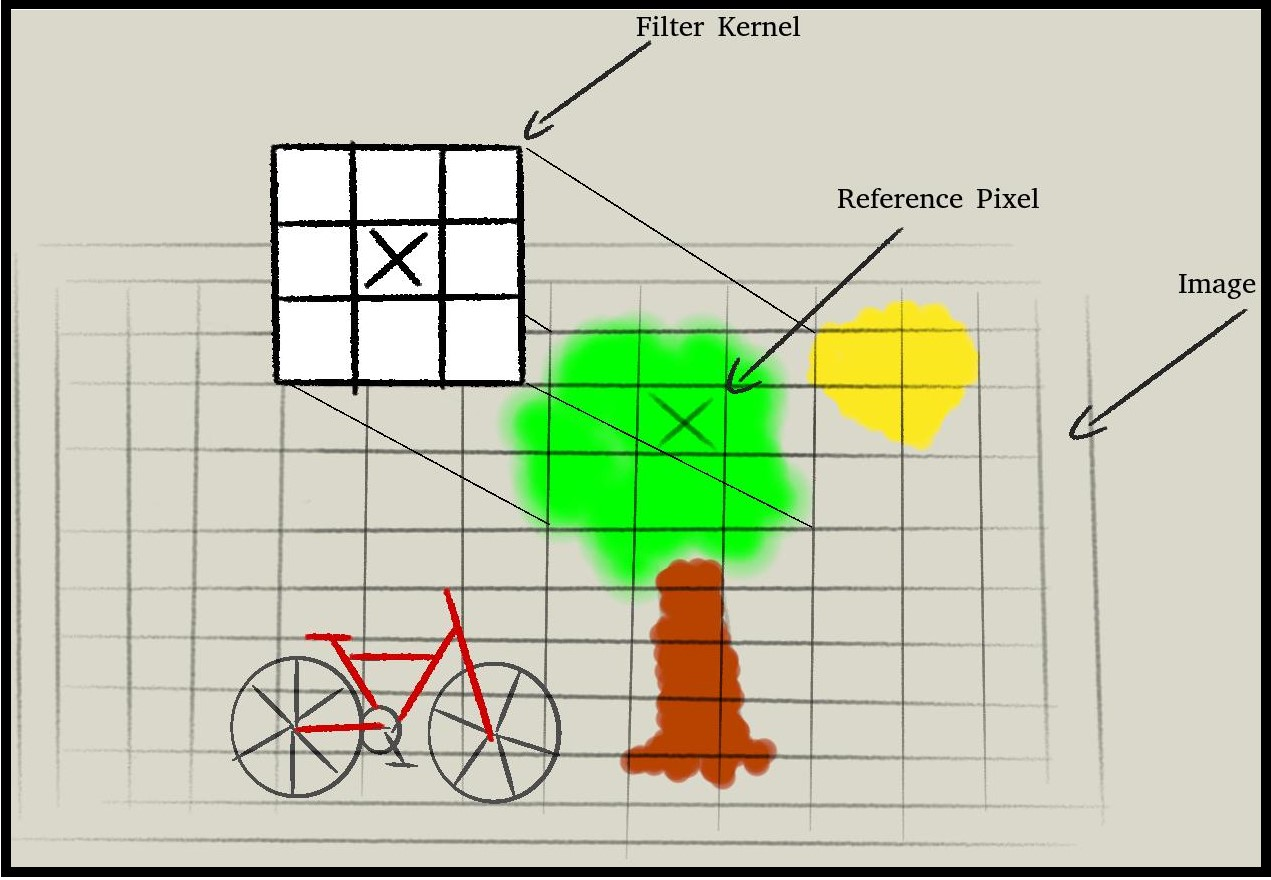
\includegraphics[width=350pt]{kernel_graphics}
 \caption{Visualization of a Filter Kernel Application}
 \label{fig:kernel_graphics}
\end{figure}

\subsubsection{Box Filter}
\label{subsubsection:boxfilter}
A box filter also known as a moving average filter simply outputs the average of its inputs because the filter weights are evenly distributed. By passing this filter over an image its sharpness is reduced giving a smoothing or blurring effect which can sometime be useful in image processing for filtering out noise. This can be observed in Figure \ref{fig:roughDog}.

% DOG BOX FILTERED%
\begin{figure}[H]
 \centering
 \begin{subfigure}[b]{0.75\textwidth}
   \centering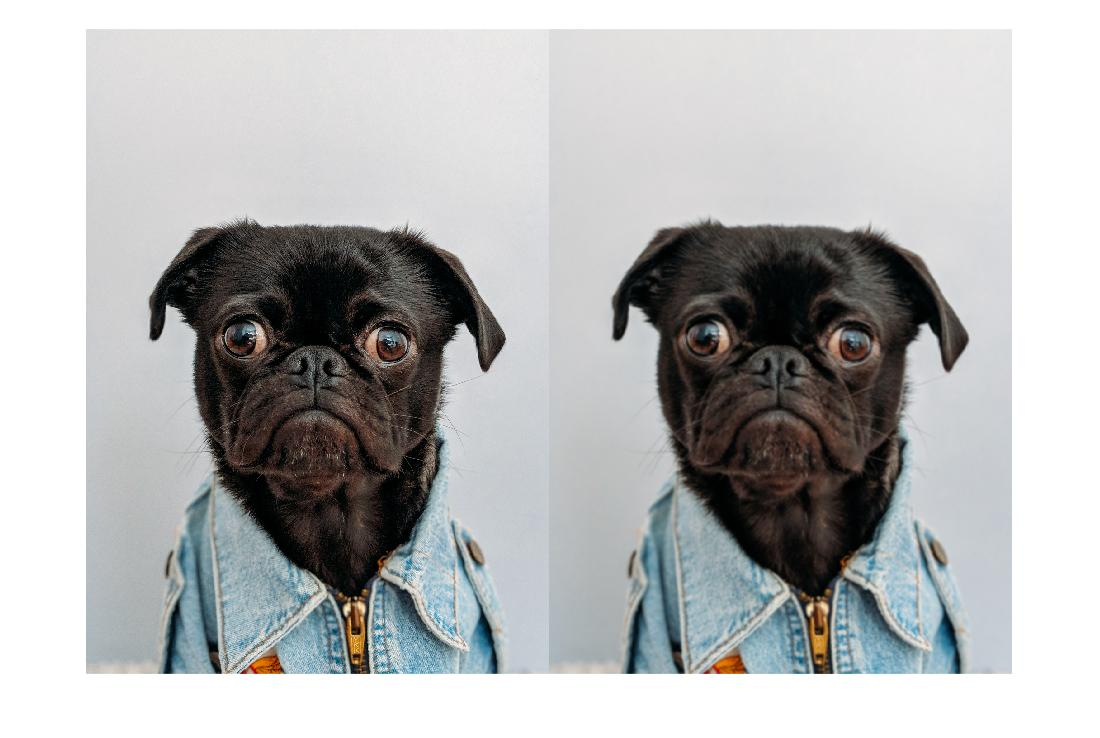
\includegraphics[width=300pt]{dogPug}
   \caption{Left: Photo by Charles Deluvio. Right: Application of $16\times16$ box filter.}
   \label{fig:roughDog}
 \end{subfigure}
 \begin{subfigure}[b]{0.25\textwidth}
   \centering
   \[
     \frac{1}{9}
   \begin{bmatrix}
      1 & 1 & 1 \\
      1 & 1 & 1 \\
      1 & 1 & 1
   \end{bmatrix}
   \]
   \caption{Box Filter Kernel.}
   \label{fig:boxkernel}
 \end{subfigure}
 \caption{Box Filter application and kernel.}
 \label{fig:boxfilter}
\end{figure}

\subsubsection{Gaussian Kernel}

The Gaussian is a rather important kernel in image processing as it models the Gaussian function (see Section \ref{section:gaussian}) or normal distribution. This filter is perhaps most well known for filtering noise but retaining edge sharpness better than other denoising filters. It works in a similar fashion to the moving average filter but as you can see in Figure XXX it is superior at filtering out the noise in comparison as it retains better edge definition. The reason the Gaussian filter is superior is because it addresses two properties about images that a generally true, 
\begin{enumerate}
    \item The actual value of a pixel is probably the same or similar to its neighbors. 
    \item Each pixel of noise in an image is added independently.
\end{enumerate}

The Gaussian which models the Normal distribution addresses both of these qualities by having high value cooefficients at the filter's center and lower values tapering out to the edges of the filter. Which essentially means values closer together are more strongly correlated than those further away from the reference pixel as can be observed in the 16x16 Gaussian filter kernel in Figure XXX.

[ Add Denoising using Gaussian Example ]
[ Add matrix of kernel filter. ]